\documentclass[20pt]{beamer}
\usepackage[orientation=portrait,size=a0,scale=1.8,debug]{beamerposter}
\mode<presentation>{\usetheme[articleid=WEPOPRPO21]{LNLS}}
\usepackage{chemformula}
\usepackage[utf8]{inputenc}
\usepackage[english]{babel} % required for rendering German special characters
\usepackage{siunitx} %pretty measurement unit rendering
\usepackage{hyperref} %enable hyperlink for urls
\usepackage{ragged2e}
\usepackage{calc}
\usepackage{datetime}
\newlength{\mylength}

\usepackage{array,booktabs,tabularx}
\newcolumntype{Z}{>{\centering\arraybackslash}X} % centered tabularx columns

\title{\huge Development of a Virtual Accelerator for Sirius}
\author{\underline{X. R. Resende}, A. H. C. Mukai, L. N. P. Vilela, I. Stevani}
\institute{Brazilian Synchrotron Light Laboratory (LNLS), Campinas, Brazil}
\date{\monthname \ \the\year}

\newlength{\abstractheight}
\setlength{\abstractheight}{15cm}

\newlength{\vaheight}
\setlength{\vaheight}{10cm}

\newlength{\columnheight}
\setlength{\columnheight}{75cm}

\begin{document}
\begin{frame}
\begin{beamercolorbox}[center]{postercolumn}
	\begin{minipage}{\textwidth}
		\parbox[t][\abstractheight]{\textwidth}{
		\begin{myblock}{\textit{Abstract}}
		A virtual accelerator is being developed for Sirius, the new 4th generation synchrotron light source being built in Campinas, Brazil.
		The virtual accelerator is an on-line beam simulator which is integrated into EPICS control system.
		It consists of a command line interface server with a channel access (CA) layer and with an in-house developed tracking code library written in C++ for efficiency gain.
		The purpose of such server is to facilitate early development and testing of high level applications for the control system.
		\end{myblock}
	}\end{minipage}
	\begin{minipage}{\textwidth}
		\parbox[t][\vaheight]{\textwidth}{
		\begin{myblock}{\textit{Virtual accelerator}}
		On-line beam simulator composed of two parts: a back-end machine
		application implementing a simulated virtual accelerator with a channel access server layer (VACA) and a set of
		front-end virtual IOCs (vIOCS) with which other control system applications interact.
		\end{myblock}
	}\end{minipage}	
\end{beamercolorbox}
\begin{columns}
	\begin{column}{0.55\textwidth}
		\begin{beamercolorbox}[center]{postercolumn}
			\begin{minipage}{.98\textwidth}  % tweaks the width, makes a new \textwidth
				\parbox[t][\columnheight]{\textwidth}{ % must be some better way to set the height, width and textwidth simultaneously
					\vspace{1cm}
					\begin{myblock}{VACA - Virtual Accelerator with Channel Access}
						\textbf{Implemented functionalities}
						\begin{itemize}
							\item Parameter-dependent current decays
							\item Closed-orbit control with dipolar correctors
							\item Beam optics variations with quadrupoles
							\item Injection and ejection that depend on magnet and timing configurations.
						\end{itemize}
						\vspace{0.5cm}
						
						\textbf{Python programming language}
						\begin{itemize}
							\item Allows for rapid development
							\item Binding layer between the CA server and a tracking code for simulations.
							\item The python package PCasPy is used as the CA server module.
							\item Trackcpp is a C++ library of beam dynamics and tracking routines developed at LNLS by the accelerator physics group. Trackcpp is converted to Python package with Swig3.0						
						\end{itemize}
						\begin{figure}
							\centering
							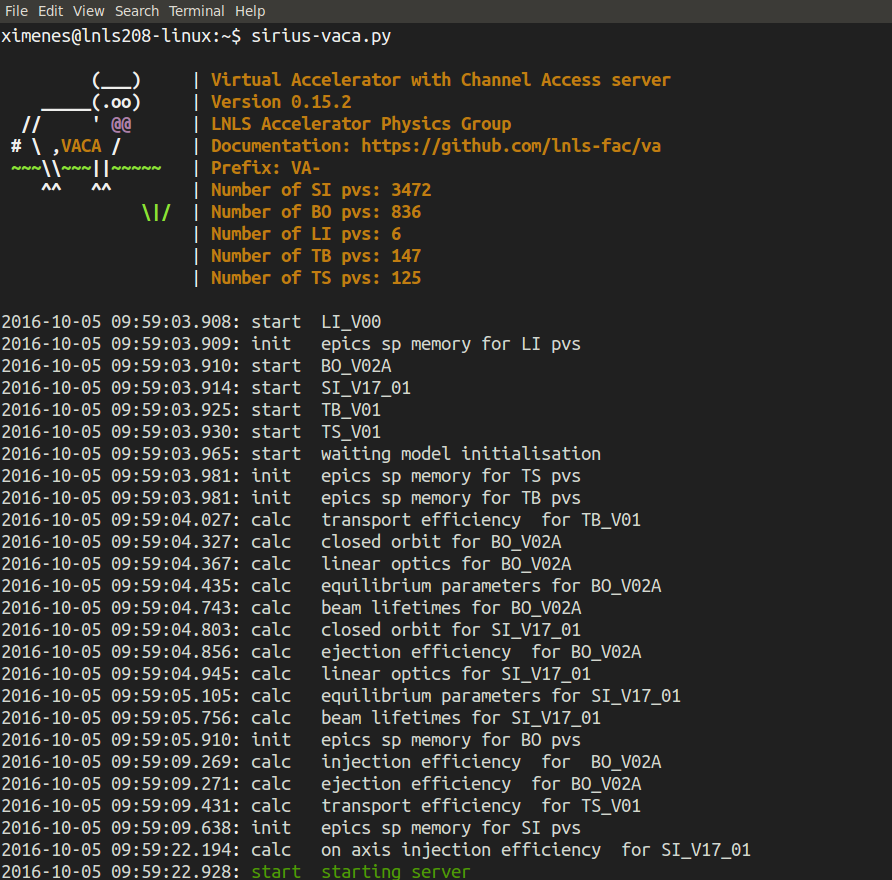
\includegraphics[width=0.855\textwidth]{../WEPOPRPO21f1.png}
							\caption{Screen printout of a command line terminal showing a running instance of VACA.}% with the display of its banner and useful information.}
						\end{figure}
					\end{myblock}
					\vspace{0.5cm}
		}\end{minipage}\end{beamercolorbox}
	\end{column}
	\begin{column}{.45\textwidth}
		\begin{beamercolorbox}[center]{postercolumn}
			\begin{minipage}{.98\textwidth} % tweaks  the width, makes a new \textwidth
				\parbox[t][\columnheight]{\textwidth}{ % must be some better way to set the the height, width and textwidth simultaneously
				\vspace{1cm}
					\begin{myblock}{Virtual IOCs}
					\begin{itemize}
					\item \textbf{si\_bpm, bo\_bpm, ts\_bpm, tb\_bpm}: they serve BPM positions that are read from VACA, adding emulated measurement fluctuations.
					\item \textbf{si\_current, bo\_current}: they provide simulated beam currents with fluctuations. %Touschek, elastic and inelastic simulated lifetimes are affected by variations of associated parameters such as RF gap voltage and reduced acceptance due to closed orbit variations.
					\item \textbf{si\_ps, bo\_ps, ts\_ps, tb\_ps}: provide read/write access to PVs that correspond to power supplies with associated magnet excitation curves.
					\item \textbf{si\_rf, bo\_rf}: implement radio frequency process variables.
					\item \textbf{si\_tune}: emulation of the tune measurement IOC.
					\item \textbf{si\_beamsize, bo\_beamsize}: emulation of beam size measurement IOC.
					\item \textbf{si\_lifetime}: emulation of lifetime calculation IOC.
					\vspace{1cm}
					\end{itemize}
					
					\end{myblock}
					\vspace{2cm}
					\begin{myblock}{Conclusions}
					
					\begin{itemize}
					\item Facilitates the development of high level applications
					\item Enables commissioning training
					\item Can be use to serve model data during Sirius operations
					\end{itemize}
					
					\vspace{2cm}
					\textbf{Future improvements}
					\begin{itemize}
					\item Details of the pulsed signals during injection and ejection processes need be considered. 
					\item Approximate coupling expressions for beam size estimates should be substituted by Ohmi's envelop formalism in trackcpp.
					%\item A cleaner separation between VACA and vIOCS is in order. 
					\item Considerations on moving from EPICS database to PCASPy for vIOCS developments. 
					\item A major revision of PV names has taken place recently and VA should be updated to contemplate the new PV naming standard.
					
					\end{itemize}
					\vspace{1cm}
					\end{myblock}
					\vspace{0.5cm}
		}\end{minipage}\end{beamercolorbox}
	\end{column}
\end{columns}
\end{frame}
\end{document}
